\باب{فوریئر تجزیہ}
\اصطلاح{دوری تفاعل}\فرہنگ{دوری!تفاعل}\فرہنگ{تفاعل!دوری}\حاشیہب{periodic function}\فرہنگ{periodic!function} سے مراد وہ تفاعل ہے جو درج ذیل مساوات پر پورا اترتا ہے جہاں \عددی{T_0}  \اصطلاح{دوری عرصہ}\فرہنگ{دوری عرصہ}\حاشیہب{time period}\فرہنگ{time period} کہلاتی ہے۔
\begin{align}
f(t)=f(t+nT_0), \quad n=\mp 1, \mp 2, \mp3, \cdots
\end{align}
درج بالا مساوات کہتی ہے کہ  کسی بھی لمحہ \عددی{t} پر دوری تفاعل کی قیمت \عددی{f(t)} اور اس لمحے سے \عددی{T_0} وقت بعد تفاعل کی قیمت \عددی{f(t+T_0)} برابر ہیں۔شکل \حوالہ{شکل_فوریئر_دوری_عرصہ} میں اس کی وضاحت  کی گئی ہے۔
\begin{figure}
\centering
\begin{tikzpicture}
\begin{axis}[kStyleCircuitsA,xtick={115,475},xticklabels={$t$,$t+T_0$},ytick=\empty]
\pgfmathsetmacro{\kt}{115}
\pgfmathsetmacro{\ktt}{\kt+360}
\addplot[domain=0:720,samples=100]{sin(x)+1/3*sin(3*x)};
\addplot[] plot coordinates {(\kt,{sin(\kt)+1/3*sin(3*\kt)+0.1}) (\kt,{sin(\kt)+1/3*sin(3*\kt)+0.3})};
\addplot[] plot coordinates {(\ktt,{sin(\ktt)+1/3*sin(3*\ktt)+0.1}) (\ktt,{sin(\ktt)+1/3*sin(3*\ktt)+0.3})};
\addplot[stealth-stealth] plot coordinates {(\kt,{sin(\kt)+1/3*sin(3*\kt)+0.2}) (\ktt,{sin(\ktt)+1/3*sin(3*\ktt)+0.2})}node[pos=0.5,fill=white]{$T_0$};
\addplot[] plot coordinates {(\kt,{sin(\kt)+1/3*sin(3*\kt)})}node[circ]{};
\addplot[] plot coordinates {(\ktt,{sin(\ktt)+1/3*sin(3*\ktt)})}node[circ]{};
\end{axis}
\end{tikzpicture}
\caption{دوری عرصہ۔}
\label{شکل_فوریئر_دوری_عرصہ}
\end{figure}
دوری عرصے کو سیکنڈ \عددی{(\si{\second})} میں ناپا جاتا ہے۔دوری عرصہ \عددی{T_0} اور \اصطلاح{تعدد}\فرہنگ{تعدد} \عددی{f_0} کا تعلق درج ذیل ہے جہاں تعدد کو \اصطلاح{ہرٹز}\فرہنگ{ہرٹز}\حاشیہب{Hertz, \si{\hertz}}\فرہنگ{Hertz}\فرہنگ{\si{\hertz}} \عددی{(\si{\hertz})} میں ناپا جاتا ہے۔
\begin{align}
f_0=\frac{1}{T_0}
\end{align}
\اصطلاح{زاویائی تعدد}\فرہنگ{زاویائی تعدد}\فرہنگ{تعدد!زاویائی} \عددی{\omega_0} اور تعدد \عددی{f_0} کا تعلق درج ذیل ہے۔
\begin{align}
\omega_0=2\pi f_0
\end{align}
زاویائی تعدد کو ریڈیئن فی سیکنڈ \عددی{(\si{\radian \per\second})} میں ناپا جاتا ہے۔شکل \حوالہ{شکل_فوریئر_چند_دوری_امواج} میں چند \اصطلاح{دوری امواج}\فرہنگ{دوری!موج}\فرہنگ{موج!دوری}\حاشیہب{periodic wave}\فرہنگ{periodic!wave} دکھائے گئے ہیں۔
\begin{figure}
\centering
\begin{subfigure}{0.5\textwidth}
\centering
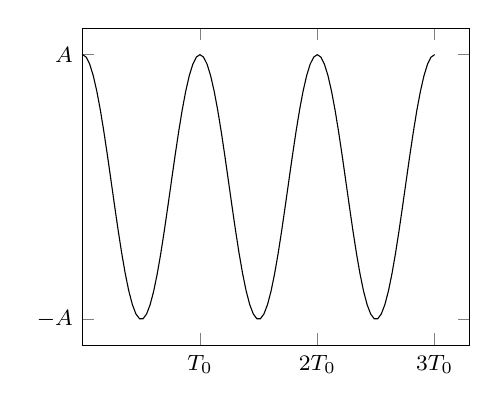
\begin{tikzpicture}
\begin{axis}[small,xmin=0,xtick={360,720,1080},xticklabels={$T_0$, $2T_0$,$3T_0$},ytick={-1,1},yticklabels={$-A$,$A$}]
\addplot[domain=0:1080,samples=100]{cos(x)};
\end{axis}
\end{tikzpicture}
\caption*{(الف) سائن نما موج۔}
\end{subfigure}%
\begin{subfigure}{0.5\textwidth}
\centering
\begin{tikzpicture}
\begin{axis}[small,xmin=0,xtick={1,3,6},xticklabels={$T_a$, $T_0$,$2T_0$},ytick={1},yticklabels={$A$}]
\addplot[] plot coordinates {(0,0) (0,1) (1,1) (1,0) (3,0) (3,1) (4,1) (4,0)(6,0) (6,1) (7,1) (7,0)};
\end{axis}%
\end{tikzpicture}
\caption*{(ب) مستطیل موج۔}
\end{subfigure}
\begin{subfigure}{0.5\textwidth}
\centering
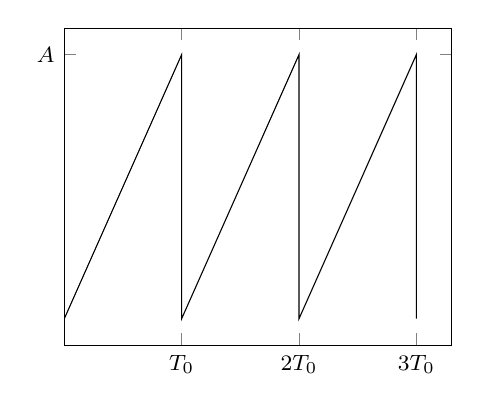
\begin{tikzpicture}
\begin{axis}[small,xmin=0,xtick={3,6,9},xticklabels={$T_0$, $2T_0$,$3T_0$},ytick={1},yticklabels={$A$}]
\addplot[] plot coordinates {(0,0) (3,1) (3,0) (6,1) (6,0) (9,1) (9,0)};
\end{axis}%
\end{tikzpicture}
\caption*{(پ) دندان موج۔}
\end{subfigure}%
\begin{subfigure}{0.5\textwidth}
\centering
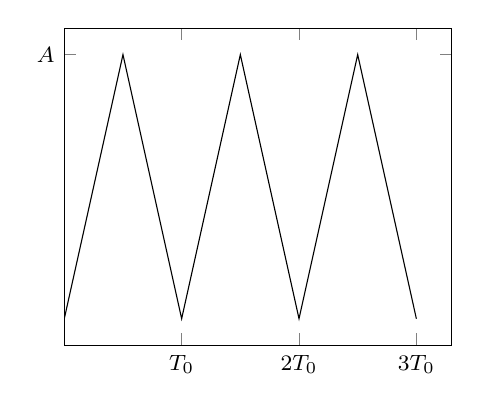
\begin{tikzpicture}
\begin{axis}[small,xmin=0,xtick={2,4,6},xticklabels={$T_0$, $2T_0$,$3T_0$},ytick={1},yticklabels={$A$}]
\addplot[] plot coordinates {(0,0) (1,1) (2,0) (3,1) (4,0) (5,1) (6,0)};
\end{axis}%
\end{tikzpicture}
\caption*{(ت) تکونی موج۔}
\end{subfigure}%
\caption{چند دوری امواج۔}
\label{شکل_فوریئر_چند_دوری_امواج}
\end{figure}

کسی بھی دوری تفاعل کو بطور درج ذیل \اصطلاح{فوریئر تسلسل}\فرہنگ{فوریئر تسلسل}\فرہنگ{تسلسل!فوریئر}\حاشیہب{Fourier series}\فرہنگ{Fourier series} لکھا\حاشیہد{جین بپٹسٹ یوسف فوریئر نے حرارتی توانائی کے بہاو پر غور کے دوران اس تسلسل کو دریافت کیا۔} جا سکتا ہے
\begin{gather}
\begin{aligned}\label{مساوات_فوریئر_تسلسل_سائن_نما_الف}
f(t)&=a_0+\sum_{n=1}^{\infty} [a_n \cos (n \omega_0 t) +b_n \sin (n \omega_0 t)]\\
&=a_0+a_1\cos \omega_0 t+a_2 \cos (2\omega_0 t)+a_3\cos (3\omega_0 t)+\cdots\\
&\phantom{=a_0\,\,}+b_1\sin \omega_0t+b_2\sin (2\omega_0t)+b_3 \sin (3\omega_0t)+\cdots
\end{aligned}
\end{gather}
جہاں \عددی{a_0}، \عددی{a_1}،\عددی{a_2}، \عددی{b_1} وغیرہ تسلسل کے \اصطلاح{عددی سر}\فرہنگ{عددی سر}\حاشیہب{coefficients}\فرہنگ{coefficients} کہلاتے ہیں۔فوریئر تسلسل کی اوسط قیمت \عددی{a_0} کے برابر ہے۔ایک دوری عرصہ \عددی{T_0} میں \عددی{\cos \omega_0 t} یا \عددی{\sin \omega_0 t} کی ایک لہر، \عددی{\cos (2\omega_0 t)} یا \عددی{\sin (2\omega_0 t)} کی دو لہریں اور \عددی{\cos (m\omega_0 t)} یا \عددی{\sin (m\omega_0 t)} کی \عددی{m} لہریں پوری آتی ہیں۔اس حقیقت کو شکل \حوالہ{شکل_فوریئر_ارکان_تعداد_فی_دوری_عرصہ} میں دکھایا گیا ہے جہاں وضاحت کی خاطر امواج کے حیطے مختلف رکھے گئے ہیں۔فوریئر تسلسل میں \عددی{a_1\cos \omega_0 t +b_1\sin \omega_0 t} \اصطلاح{بنیادی رکن}\فرہنگ{بنیادی رکن}\فرہنگ{ہارمونی!بنیادی رکن}\حاشیہب{fundamental component}\فرہنگ{fundamental component} یا \اصطلاح{بنیادی جزو} کہلاتا ہے،   \عددی{a_2\cos (2\omega_0 t) +b_2\sin (2\omega_0 t)} \اصطلاح{دوسرا ہارمونی رکن}\فرہنگ{دوسرا ہارمونی رکن}\فرہنگ{ہارمونی!دوسرا رکن}\حاشیہب{second harmonic}\فرہنگ{harmonic!second} کہلاتا ہے،  \عددی{a_3\cos (3\omega_0 t) +b_3\sin (3\omega_0 t)} تیسرا ہارمونی رکن اور اسی طرح \عددی{a_m\cos (m\omega_0 t) +b_m\sin (m\omega_0 t)} ایم ہارمونی رکن کہلاتا ہے۔
\begin{figure}
\centering
\begin{tikzpicture}
\begin{axis}[kStyleCircuitsA,xlabel={$t\,(\si{\second})$},xtick={90,180,270,360},xticklabels={$\frac{1}{4}T_0$,$\frac{1}{2}T_0$,$\frac{3}{2}T_0$,$T_0$},ytick={1,-1},yticklabels={$+A_0$,$-A_0$}]
\addplot[mark=none,color=black,domain=0:360,samples=100]{sin(x)}node[pos=0.4,pin=45:{$A_0\sin \omega_0 t$}]{};
\addplot[mark=none,color=black,domain=0:360,samples=100]{0.5*sin(2*x)}node[pos=0.7,pin=45:{$\frac{A_0}{2}\sin 2\omega_0 t$}]{};
\end{axis}
\end{tikzpicture}
\caption{ایک دوری عرصہ میں فوریئر تسلسل کے ارکان کی تعداد۔}
\label{شکل_فوریئر_ارکان_تعداد_فی_دوری_عرصہ}
\end{figure}
%======================
ہم یہاں اصل رک کر چند حقائق اور تکملات پر غور کرتے ہیں جو فوریئر تسلسل میں کلیدی کردار ادا کرتے ہیں۔

آپ دو سمتیوں کے \اصطلاح{نقطہ ضرب}\فرہنگ{نقطہ ضرب}\فرہنگ{ضرب!نقطہ}\حاشیہب{dot product}\فرہنگ{dot product} سے خوب واقف ہیں۔سمتیہ \سمتیہ{A} اور \سمتیہ{B} کا نقطہ ضرب یا \اصطلاح{غیر سمتی ضرب}\فرہنگ{غیر سمتی ضرب}\فرہنگ{ضرب!غیر سمتی}\حاشیہب{scalar product}\فرہنگ{scalar product} درج ذیل ہے جہاں دونوں سمتیوں کے مابین زاویہ \عددی{\theta} ہے۔
\begin{align}
\kvec{A} \cdot \kvec{B}=A B \cos \theta
\end{align} 
آپس میں \اصطلاح{عمودی}\فرہنگ{عمودی}\حاشیہب{orthogonal}\فرہنگ{orthogonal} سمتیوں کے مابین \عددی{\theta=90^{\circ}} ہونے کی بدولت \عددی{\kvec{A} \cdot \kvec{B}=0} ہوتا ہے جبکہ کسی بھی سمتیہ کے خود نقطہ ضرب کا جذر اس کے حیطے  کے برابر ہوتا ہے۔
\begin{gather}
\begin{aligned}
 \abs{\kvec{A}}=\sqrt{\kvec{A} \cdot \kvec{A}}
\end{aligned}
\end{gather}
اسی سوچ کے ساتھ تفاعل کا نقطہ ضرب بیان کیا جاتا ہے۔

اگر تفاعل \عددی{f(t) \ne 0} اور \عددی{g(t)\ne 0} کے حاصل ضرب کا تکمل \عددی{a \le t \le b} فاصلے پر صفر کے برابر ہو
\begin{align}
\int_a^b f(t)g(t) \dif t=0
\end{align}
تو \عددی{a\le t\le b} فاصلے پر ان تفاعل کو آپس میں \اصطلاح{عمودی} تصور کیا جاتا ہے۔یاد رہے کہ دونوں تفاعل از خود \اصطلاح{غیر سمتی}\فرہنگ{غیر سمتی}\حاشیہب{scalar}\فرہنگ{scalar} اور غیر صفر ہیں۔

کسی بھی مقدار کا مربع مثبت ہوتا ہے لہٰذا تفاعل کا مربع \عددی{f^2(t)} ہر نقطے پر مثبت ہو گا۔ فاصلہ \عددی{a \le t \le b}  پر تفاعل کے \اصطلاح{معیار}\فرہنگ{معیار}\حاشیہب{norm}\فرہنگ{norm} \عددی{\parallel f(t) \parallel} سے مراد 
\begin{align}
\parallel f(t) \parallel =\sqrt{\int_a^b f^2(t) \dif t}
\end{align}
ہے۔
%===================
\ابتدا{مثال}
ثابت کریں کہ \عددی{0 \le t \le T_0}  فاصلے پر \عددی{\cos (m\omega_0 t)} اور \عددی{\cos (n\omega_0 t)} آپس میں عمودی ہیں جہاں \عددی{m=1,2,3,\cdots} اور \عددی{n=1,2,3,\cdots} ممکن ہیں لیکن \عددی{m\ne n} ہے۔

حل:دیے گئے فاصلے پر دونوں تفاعل کے حاصل ضرب کا تکمل لیتے ہیں۔
\begin{align*}
\int_0^{T_0} \cos (m\omega_0 t) \cos (n\omega_0 t) \dif t&=\int_0^{T_0} \frac{\cos\left[(m+n)\frac{2\pi}{T_0} t\right]+\cos\left[(m-n)\frac{2\pi}{T_0} t\right]}{2}\dif t\\
&=\left.\frac{\sin\left[(m+n)\frac{2\pi}{T_0} t\right]}{2(m+n)\frac{2\pi}{T_0} }+\frac{\sin\left[(m-n)\frac{2\pi}{T_0} t\right]}{2(m-n)\frac{2\pi}{T_0} }\right|_0^{T_0}\\
&=\frac{\sin[(m+n)2\pi]}{2(m+n)\frac{2\pi}{T_0} }+\frac{\sin[(m-n)2\pi]}{2(m-n)\frac{2\pi}{T_0} }\\
&\quad \quad \quad \quad -\frac{\sin[(m+n)0]}{2(m+n)\frac{2\pi}{T_0} }-\frac{\sin[(m-n)0]}{2(m-n)\frac{2\pi}{T_0} }
\end{align*}
چونکہ \عددی{m} اور \عددی{n} عدد صحیح ہیں لہٰذا \عددی{m+n} اور \عددی{m-n} بھی عدد صحیح ہوں گے لہٰذا \عددی{\sin[(m+n)2\pi]=0} اور \عددی{\sin[(m-n)2\pi]=0}  ہوں گے۔اس طرح درج ذیل حاصل ہوتا ہے جو عمودی تفاعل کو ظاہر کرتی ہے۔
\begin{align}\label{مساوات_فوریئر_مختلف_تکمل_الف}
\int_0^{T_0} \cos (m\omega_0 t) \cos (n\omega_0 t) \dif t=0\quad (m\ne n)
\end{align}
\انتہا{مثال}
%===================

\ابتدا{مثال}
ثابت کریں کہ \عددی{0 \le t \le T_0} فاصلے پر \عددی{\sin (m\omega_0 t)} اور \عددی{\sin (n\omega_0 t)} آپس میں عمودی ہیں جہاں \عددی{m=1,2,3,\cdots} اور \عددی{n=1,2,3,\cdots} ممکن ہیں لیکن \عددی{m\ne n} ہے۔

حل:دیے گئے فاصلے پر دونوں تفاعل کے حاصل ضرب کا تکمل لیتے ہیں۔
\begin{align*}
\int_0^{T_0} \sin (m\omega_0 t) \sin (n\omega_0 t) \dif t&=\int_0^{T_0} \frac{\cos\left[(m-n)\frac{2\pi}{T_0} t\right]-\cos\left[(m+n)\frac{2\pi}{T_0} t\right]}{2}\dif t\\
&=\left.\frac{\sin\left[(m-n)\frac{2\pi}{T_0} t\right]}{2(m-n)\frac{2\pi}{T_0} }-\frac{\sin\left[(m+n)\frac{2\pi}{T_0} t\right]}{2(m+n)\frac{2\pi}{T_0} }\right|_0^{T_0}\\
&=\frac{\sin[(m-n)2\pi]}{2(m-n)\frac{2\pi}{T_0} }-\frac{\sin[(m+n)2\pi]}{2(m+n)\frac{2\pi}{T_0} }\\
&\quad \quad \quad \quad -\frac{\sin[(m-n)0]}{2(m-n)\frac{2\pi}{T_0} }+\frac{\sin[(m+n)0]}{2(m+n)\frac{2\pi}{T_0} }
\end{align*}
چونکہ \عددی{m} اور \عددی{n} عدد صحیح ہیں لہٰذا \عددی{m+n} اور \عددی{m-n} بھی عدد صحیح ہوں گے لہٰذا \عددی{\sin[(m+n)2\pi]=0} اور \عددی{\sin[(m-n)2\pi]=0}  ہوں گے۔اس طرح درج ذیل حاصل ہوتا ہے جو عمودی تفاعل کو ظاہر کرتی ہے۔
\begin{align}\label{مساوات_فوریئر_مختلف_تکمل_ب}
\int_0^{T_0} \sin (m\omega_0 t) \sin (n\omega_0 t) \dif t=0\quad (m\ne n)
\end{align}
\انتہا{مثال}
%===================

\ابتدا{مثال}
ثابت کریں کہ \عددی{0 \le t \le T_0} فاصلے پر \عددی{\cos (m\omega_0 t)} اور \عددی{\sin (n\omega_0 t)} آپس میں عمودی ہیں جہاں \عددی{m=1,2,3,\cdots} اور \عددی{n=1,2,3,\cdots} ممکن ہیں۔

حل:دیے گئے فاصلے پر دونوں تفاعل کے حاصل ضرب کا تکمل لیتے ہیں۔
\begin{align*}
\int_0^{T_0} \cos (m\omega_0 t) \sin (n\omega_0 t) \dif t&=\frac{1}{2}\int_0^{T_0} \sin\left[(m+n)\frac{2\pi}{T_0} t\right]-\sin\left[(m-n)\frac{2\pi}{T_0} t\right]\dif t\\
&=\left.-\frac{\cos\left[(m+n)\frac{2\pi}{T_0} t\right]}{2(m+n)\frac{2\pi}{T_0}}+\frac{\cos\left[(m-n)\frac{2\pi}{T_0} t\right]}{2(m-n)\frac{2\pi}{T_0}}\right|_0^{T_0}\\
&=-\frac{\cos[(m+n)2\pi]}{2(m+n)\frac{2\pi}{T_0}}+\frac{\cos[(m-n)2\pi]}{2(m-n)\frac{2\pi}{T_0}}\\
&\quad \quad \quad \quad +\frac{\cos[(m+n)0]}{2(m+n)\frac{2\pi}{T_0}}-\frac{\cos[(m-n)0]}{2(m-n)\frac{2\pi}{T_0}}
\end{align*}
چونکہ \عددی{m} اور \عددی{n} عدد صحیح ہیں لہٰذا \عددی{m+n} اور \عددی{m-n} بھی عدد صحیح ہوں گے لہٰذا \عددی{\cos(m+n)2\pi=1} اور \عددی{\cos(m-n)2\pi=1}  ہوں گے۔اس طرح درج ذیل حاصل ہوتا ہے جو عمودی تفاعل کو ظاہر کرتی ہے۔
\begin{align}\label{مساوات_فوریئر_مختلف_تکمل_پ}
\int_0^{T_0} \cos (m\omega_0 t) \sin (n\omega_0 t) \dif t=0\quad (m\ne n)
\end{align}
\انتہا{مثال}
%===================
\ابتدا{مثال}
تفاعل \عددی{f(t)=\cos (m\omega_0 t)} کا معیار \عددی{0 \le t \le T_0} فاصلے پر حاصل کریں جہاں  \عددی{{m=1,2,3,\cdots}} ممکن ہے۔ 

حل:دیے گئے فاصلے پر معیار کو تکمل سے حاصل کرتے ہیں۔
\begin{align*}
\parallel f(t) \parallel^2&=\int_0^{T_0} \cos^2 \left(m\frac{2\pi}{T_0} t\right) \dif t\\
&=\frac{1}{2}\int_0^{T_0}\left[ 1+\cos \left(2m\frac{2\pi}{T_0} t\right)\right] \dif t\\
&=\left. \frac{t}{2}+\frac{\sin \left(2m\frac{2\pi}{T_0} t\right)}{4m\frac{2\pi}{T_0}}\right|_0^{T_0}\\
&=\frac{T_0}{2}+\frac{\sin 4m\pi}{4m\frac{2\pi}{T_0}}-\frac{0}{2}-\frac{\sin 0}{4m\frac{2\pi}{T_0}}\\
&=\frac{T_0}{2}
\end{align*}
دونوں اطراف کا جذر لیتے ہوئے  \عددی{0 \le t \le T_0} فاصلے پر معیار ملتا ہے۔
\begin{align}\label{مساوات_فوریئر_مختلف_تکمل_ت}
\parallel \cos (m\omega_0 t) \parallel =\sqrt{\int_0^{T_0} \cos^2  (m\omega_0 t) \dif t}=\sqrt{\frac{T_0}{2}}
\end{align}
\انتہا{مثال}
%==================

\ابتدا{مشق}
تفاعل \عددی{f(t)=\sin m\omega_0 t} کا معیار \عددی{0 \le t \le T_0} فاصلے پر درج ذیل ہے جہاں \عددی{m=1,2,3,\cdots} ممکن ہے۔ اس معیار کو حاصل کریں۔
\begin{align}\label{مساوات_فوریئر_مختلف_تکمل_ٹ}
\parallel \sin (m\omega_0 t) \parallel =\sqrt{\int_0^{T_0} \sin^2 (m\omega_0 t) \dif t}=\sqrt{\frac{T_0}{2}}
\end{align}
\انتہا{مشق}
%==================
\ابتدا{مشق}
درج ذیل دو مساوات کو ثابت کریں جہاں \عددی{m=1,2,3,\cdots} ممکن ہے۔
\begin{align}
\int_0^{T_0} \cos (m\omega_0 t) \dif t&=0 \label{مساوات_فوریئر_مختلف_تکمل_ث}\\
\int_0^{T_0} \sin (m\omega_0 t) \dif t&=0\label{مساوات_فوریئر_مختلف_تکمل_ج}
\end{align}
\انتہا{مشق}
%====================
مساوات \حوالہ{مساوات_فوریئر_مختلف_تکمل_الف}، مساوات \حوالہ{مساوات_فوریئر_مختلف_تکمل_ب} اور مساوات \حوالہ{مساوات_فوریئر_مختلف_تکمل_پ} مل کر ثابت کرتے ہیں کہ فوریئر تسلسل میں استعمال ہونے والا ہر تفاعل بقایا تمام تفاعل کے ساتھ \عددی{0 \le t \le T_0} فاصلے پر عمودی ہے۔یوں \عددی{\cos 3\omega_0 t} کو مثال بناتے ہوئے ہم دیکھتے ہیں کہ یہ \عددی{\cos (\omega_0 t)}، \عددی{\cos(2\omega_0 t)}،\عددی{\cos(4\omega_0 t)}، \عددی{\sin(\omega_0 t)}، \عددی{\sin(2\omega_0 t)}، \عددی{\sin(3\omega_0 t)} وغیرہ کے ساتھ عمودی ہے۔

%====================
درج بالا تکملات حاصل کرنے کے بعد اصل مضمون یعنی فوریئر تسلسل پر دوبارہ آتے ہیں۔مساوات \حوالہ{مساوات_فوریئر_مختلف_تکمل_الف} تا مساوات \حوالہ{مساوات_فوریئر_مختلف_تکمل_ج} کو استعمال کرتے ہوئے مساوات  \حوالہ{مساوات_فوریئر_تسلسل_سائن_نما_الف} کے عددی سر \عددی{a_0, a_1,a_2,b_1,\cdots} حاصل کئے جا سکتے ہیں۔آئیں ایسا ہی کریں۔

عددی سر \عددی{a_0} کی قیمت دریافت کرنے کی خاطر ہم  مساوات  \حوالہ{مساوات_فوریئر_تسلسل_سائن_نما_الف} کا تکمل \عددی{0 \le t \le T_0} فاصلے پر لیتے ہیں
\begin{align*}
\int_0^{T_0}f(t) \dif t&=\int_0^{T_0} a_0 \dif t+\sum_{n=1}^{\infty}  \int_0^{T_0}(a_n\cos n \omega_0 t +b_n \sin n \omega_0 t) \dif t\\
&=a_0 T_0
\end{align*}
جہاں مساوات \حوالہ{مساوات_فوریئر_مختلف_تکمل_ث} اور مساوات \حوالہ{مساوات_فوریئر_مختلف_تکمل_ج} کو استعمال کرتے ہوئے مجموعے میں دیے تمام تکمل کو صفر کے برابر پر کیا گیا ہے۔ یوں درج ذیل حاصل ہوتا ہے۔
\begin{align}\label{مساوات_فوریئر_عددی_سر_الف}
a_0=\frac{1}{T_0}\int_0^{T_0}f(t) \dif t
\end{align}
مساوات \حوالہ{مساوات_فوریئر_عددی_سر_الف} کہتا ہے کہ \عددی{a_0} تفاعل \عددی{f(t)} کی اوسط قیمت ہے۔


عددی سر \عددی{a_m} حاصل کرنے کی خاطر مساوات \حوالہ{مساوات_فوریئر_تسلسل_سائن_نما_الف} کے دونوں اطراف کو \عددی{\cos (m\omega_0t)} سے ضرب دیتے ہوئے ایک دوری عرصے پر تکمل کرتے ہیں۔ہم تکمل کو \عددی{0 \le t \le T_0} پر حاصل کرتے ہیں۔
\begin{multline}\label{مساوات_فوریئر_عددی_سر_کا_حصول_الف}
\int_0^{T_0}f(t) \cos( m \omega_0 t) \dif t=\\
\int_0^{T_0} a_0 \cos (m\omega_0 t) \dif t+\sum_{n=1}^{\infty}  \int_0^{T_0} a_n\cos (n \omega_0 t)  \cos (m \omega_0 t) \dif t \\
+\sum_{n=1}^{\infty} \int_0^{T_0} b_n \sin (n \omega_0 t) \cos (m\omega_0 t) \dif t
\end{multline}
دائیں ہاتھ پہلا تکمل مساوات \حوالہ{مساوات_فوریئر_مختلف_تکمل_ث} کی بنا صفر کے برابر ہے جبکہ مساوات \حوالہ{مساوات_فوریئر_مختلف_تکمل_پ} کے تحت تیسرا تکمل صفر کے برابر ہے۔آئیں دوسرے تکمل پر غور کریں۔
\begin{multline*}
\sum_{n=1}^{\infty}  \int_0^{T_0} a_n\cos n \omega_0 t  \cos m \omega_0 t \dif t =\\
\int_0^{T_0} \cos (m\omega_0 t)\left[a_1 \cos \omega_0 t+a_2\cos (2\omega_0 t)+\cdots \right.\\
\left.+a_{m-1}\cos[(m-1)\omega_0 t]+a_m\cos(m\omega_0 t)+\cdots \right] \dif t
\end{multline*}
اب اگر \عددی{n \ne m} ہو تب مساوات \حوالہ{مساوات_فوریئر_مختلف_تکمل_الف} کے تحت تکمل صفر کے برابر ہو گا۔البتہ \عددی{n=m} کی صورت میں مساوات \حوالہ{مساوات_فوریئر_مختلف_تکمل_ت} کو استعمال کرتے ہوئے
\begin{align*}
\int_0^{T_0}a_m \cos^2 (m\omega_0 t) \dif t=a_m\frac{T_0}{2}
\end{align*} 
حاصل ہوتا ہے۔ان قیمتوں کو مساوات \حوالہ{مساوات_فوریئر_عددی_سر_کا_حصول_الف} میں پر کرتے ہوئے درج ذیل حاصل ہوتا ہے۔
\begin{align}\label{مساوات_فوریئر_عددی_سر_ب}
a_m=\frac{2}{T_0}\int_0^{T_0}f(t) \cos (m \omega_0 t) \dif t
\end{align}

عددی سر \عددی{b_m} حاصل کرنے کی خاطر مساوات \حوالہ{مساوات_فوریئر_تسلسل_سائن_نما_الف} کے دونوں اطراف کو \عددی{\sin (m\omega_0 t)} سے ضرب دیتے ہوئے ایک دوری عرصے پر تکمل کرتے ہیں۔ہم تکمل کو \عددی{0 \le t \le T_0} پر حاصل کرتے ہیں۔
\begin{multline}\label{مساوات_فوریئر_عددی_سر_کا_حصول_ب}
\int_0^{T_0}f(t) \sin (m \omega_0 t) \dif t=\\
\int_0^{T_0} a_0 \sin (m\omega_0 t) \dif t+\sum_{n=1}^{\infty}  \int_0^{T_0} a_n\cos (n \omega_0 t)  \sin (m \omega_0 t) \dif t \\
+\sum_{n=1}^{\infty} \int_0^{T_0} b_n \sin (n \omega_0 t) \sin (m\omega_0 t) \dif t
\end{multline}
دائیں ہاتھ پہلا تکمل مساوات \حوالہ{مساوات_فوریئر_مختلف_تکمل_ج} کی بنا صفر کے برابر ہے جبکہ مساوات \حوالہ{مساوات_فوریئر_مختلف_تکمل_پ} کے تحت دوسرا تکمل صفر کے برابر ہے۔آئیں تیسرے تکمل پر غور کریں۔
\begin{multline*}
\sum_{n=1}^{\infty} \int_0^{T_0} b_n \sin (n \omega_0 t) \sin (m\omega_0 t) \dif t=\\
\int_0^{T_0} \sin (m\omega_0 t)\left[b_1 \sin \omega_0 t+b_2\sin (2\omega_0 t)+\cdots \right.\\
\left.+b_{m-1}\sin[(m-1)\omega_0 t]+b_m\sin(m\omega_0 t)+\cdots \right] \dif t
\end{multline*}
اب اگر \عددی{n \ne m} ہو تب مساوات \حوالہ{مساوات_فوریئر_مختلف_تکمل_ب} کے تحت تکمل صفر کے برابر ہو گا۔البتہ \عددی{n=m} کی صورت میں مساوات \حوالہ{مساوات_فوریئر_مختلف_تکمل_ٹ} کو استعمال کرتے ہوئے
\begin{align*}
\int_0^{T_0}b_m \sin^2 (m\omega_0 t) \dif t=b_m\frac{T_0}{2}
\end{align*} 
حاصل ہوتا ہے۔ان قیمتوں کو مساوات \حوالہ{مساوات_فوریئر_عددی_سر_کا_حصول_الف} میں پر کرتے ہوئے درج ذیل حاصل ہوتا ہے۔
\begin{align}\label{مساوات_فوریئر_عددی_سر_پ}
b_m=\frac{2}{T_0}\int_0^{T_0}f(t) \sin (m \omega_0 t) \dif t
\end{align}
مساوات \حوالہ{مساوات_فوریئر_عددی_سر_الف}، مساوات \حوالہ{مساوات_فوریئر_عددی_سر_ب} اور مساوات \حوالہ{مساوات_فوریئر_عددی_سر_پ} فوریئر تکمل کے عددی سر دیتے ہیں۔انہیں یہاں اکٹھے پیش کرتے ہیں۔
\begin{gather}
\begin{aligned}\label{مساوات_فوریئر_عددی_سر_ت}
a_0&=\frac{1}{T_0}\int_0^{T_0}f(t) \dif t\\
a_m&=\frac{2}{T_0}\int_0^{T_0}f(t) \cos (m \omega_0 t) \dif t\\
b_m&=\frac{2}{T_0}\int_0^{T_0}f(t) \sin (m \omega_0 t) \dif t
\end{aligned}
\end{gather}
%============

\ابتدا{مثال}\شناخت{مثال_فوریئر_دندان_موج_الف}
شکل \حوالہ{شکل_فوریئر_دندان_موج_الف} میں دکھائے گئے \اصطلاح{دندان موج}\فرہنگ{دندان موج}\فرہنگ{موج!دندان}\فرہنگ{saw tooth} کا فوریئر تسلسل حاصل کریں۔دو، تین اور دس فوریئر ارکان استعمال کرتے ہوئے  موج کا خط کھینچیں۔آپ دیکھ سکتے ہیں کہ موج کا دوری عرصہ \عددی{T_0=\SI{3}{\second}} ہے۔
\begin{figure}
\centering
\begin{subfigure}{0.5\textwidth}
\centering
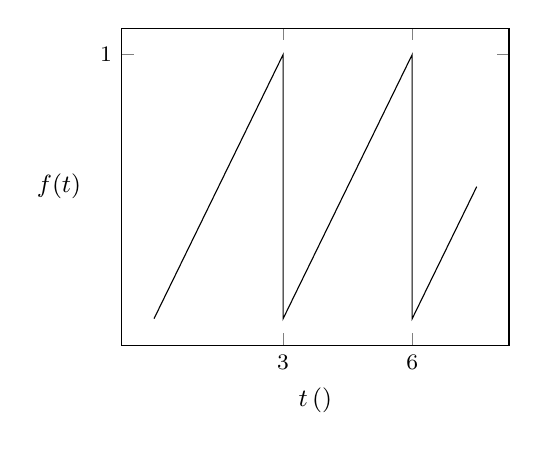
\begin{tikzpicture}
\begin{axis}[small,xlabel={$t\,(\second)$},ylabel={$f(t)$},ylabel style={rotate=-90},xtick={3,6},xticklabels={$3$,$6$},ytick={1},yticklabels={$1$}]
\addplot[] plot coordinates {(0,0)  (3,1)  (3,0) (6,1) (6,0) (7.5,0.5)};
\end{axis}
\end{tikzpicture}
\caption*{(الف)}
\end{subfigure}%
\begin{subfigure}{0.5\textwidth}
\centering
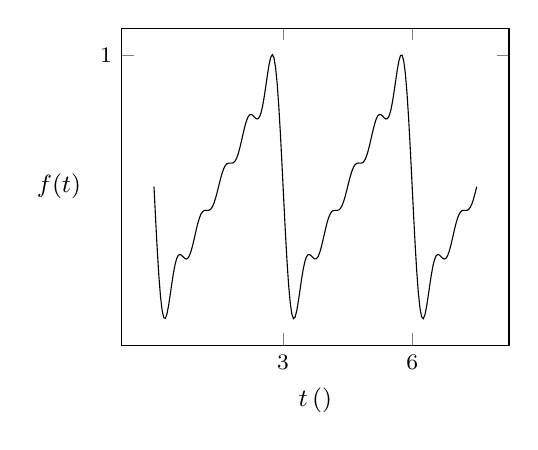
\begin{tikzpicture}
\begin{axis}[small,xlabel={$t\,(\second)$},ylabel={$f(t)$},ylabel style={rotate=-90},xtick={3,6},xticklabels={$3$,$6$},ytick={1},yticklabels={$1$}]
\addplot[domain=0:7.5,samples=200]{1/2-1/pi*(sin(120*x)+1/2*sin(2*120*x)+1/3*sin(3*120*x)+1/4*sin(4*120*x)+1/5*sin(5*120*x))}; 
\end{axis}
\end{tikzpicture}
\caption*{(ب)}
\end{subfigure}%
\caption{مثال \حوالہ{مثال_فوریئر_دندان_موج_الف} کی دندان موج۔}
\label{شکل_فوریئر_دندان_موج_الف}
\end{figure}

حل:شکل میں دکھائی گئی موج \عددی{(0,0)} سے \عددی{(3,1)} تک بالکل سیدھی لکیر کی مانند ہے جس کی ڈھلوان 
\begin{align*}
\text{ڈھلوان}=\frac{y_2-y_1}{x_2-x_1}=\frac{1-0}{3-0}=\frac{1}{3}
\end{align*}
ہے لہٰذا اس سیدھے حصے کی مساوات درج ذیل لکھی جا سکتی ہے جہاں لکیر پر کسی بھی نقطے کے کارتیسی محدد مساوات میں پر کرنے سے \عددی{c} کی قیمت حاصل کی جا سکتی ہے۔
\begin{align*}
y=\frac{x}{3}+c
\end{align*}
ہم درج بالا میں \عددی{(0,0)} پر کرتے ہوئے
\begin{align*}
0=\frac{0}{3}+c
\end{align*}
 \عددی{c=0} حاصل کرتے ہیں لہٰذا سیدھی حصے کی مساوات \عددی{y=\tfrac{x}{3}} یعنی
\begin{align}
f(t)=\frac{t}{3}
\end{align}
ہے جہاں کارتیسی نظام کے \عددی{x} محور پر \عددی{t} اور \عددی{y} محور پر \عددی{f(t)} پر کئے گئے ہیں۔

مساوات \حوالہ{مساوات_فوریئر_عددی_سر_ت} سے فوریئر تسلسل کے عددی سر حاصل کرتے ہیں۔
\begin{align*}
a_0&=\frac{1}{T_0}\int_0^{T_0} f(t) \dif t\\
&=\frac{1}{3}\int_0^3 \frac{t}{3} \dif t\\
&=\left. \frac{1}{3} \frac{t^2}{6} \right|_0^3\\
&=\frac{1}{2}
\end{align*}
چونکہ \عددی{a_0} تفاعل کی اوسط قیمت کے برابر ہے لہٰذا یہی جواب تکون کے رقبے \عددی{\tfrac{1}{2}\times 3\times 1=\tfrac{3}{2}} اور قاعدہ \عددی{3} سے حاصل کی جا سکتی ہے یعنی
\begin{align*}
\text{اوسط}&=\frac{\text{رقبہ}}{\text{قاعدہ}}=\frac{\frac{3}{2}}{3}=\frac{1}{2}
\end{align*}
عددی سر \عددی{a_m} حاصل کرتے ہیں۔
\begin{align*}
a_m&=\frac{2}{T_0}\int_0^{T_0} f(t)\cos (m\omega_0 t) \dif t\\
&=\frac{2}{3}\int_0^3 \frac{t}{3} \cos (m \frac{2\pi}{3} t) \dif t\\
&=\left. \frac{2}{9}t \frac{\sin(\frac{2\pi}{3}mt)}{\frac{2\pi}{3}m}+\frac{2}{9}\frac{\cos(\frac{2\pi}{3}mt)}{\left(\frac{2\pi}{3}m\right)^2}\right|_0^3\\
&=0
\end{align*}
اس کا مطلب ہے کہ دندان موج کی فوریئر تسلسل میں کوئی کوسائن تفاعل نہیں پایا جاتا۔

عددی سر \عددی{b_m} حاصل کرتے ہیں۔
\begin{align*}
b_m&=\frac{2}{T_0}\int_0^{T_0} f(t)\sin(m\omega_0 t) \dif t\\
&=\frac{2}{3}\int_0^3 \frac{t}{3}\sin (m\frac{2\pi}{3} t) \dif t\\
&=\left.-\frac{2}{9}t\frac{\cos(\frac{2\pi}{3}mt)}{\frac{2\pi}{3}m}+\frac{2}{9}\frac{\sin(\frac{2\pi}{3}mt)}{\left(\frac{2\pi}{3}m\right)^2}\right|_0^3\\
&=-\frac{1}{m\pi}
\end{align*}
یوں \عددی{m=1,2,3,\cdots} پر کرتے ہوئے عددی سر حاصل ہوتے ہیں یعنی
\begin{align*}
b_1&=-\frac{1}{\pi}\\
b_2&=-\frac{1}{2\pi}\\
b_3&=-\frac{1}{3\pi}\\
&\vdots
\end{align*}
لہٰذا فوریئر تسلسل درج ذیل لکھی جائے گی۔
\begin{align}
f(t)=\frac{1}{2}-\frac{1}{\pi}\left[\sin \omega_0 t+\frac{1}{2} \sin (2\omega_0 t) +\frac{1}{3} \sin (3\omega_0 t)+\cdots\right]
\end{align}
\انتہا{مثال}
